% Counts checked against saved case-level evaluations; lengths show trajectory counts.
\begingroup
\definecolor{direct}{HTML}{24557A}
\definecolor{recovery}{HTML}{168475}
\definecolor{semantic}{HTML}{E4B15A}
\definecolor{execution}{HTML}{A34C40}
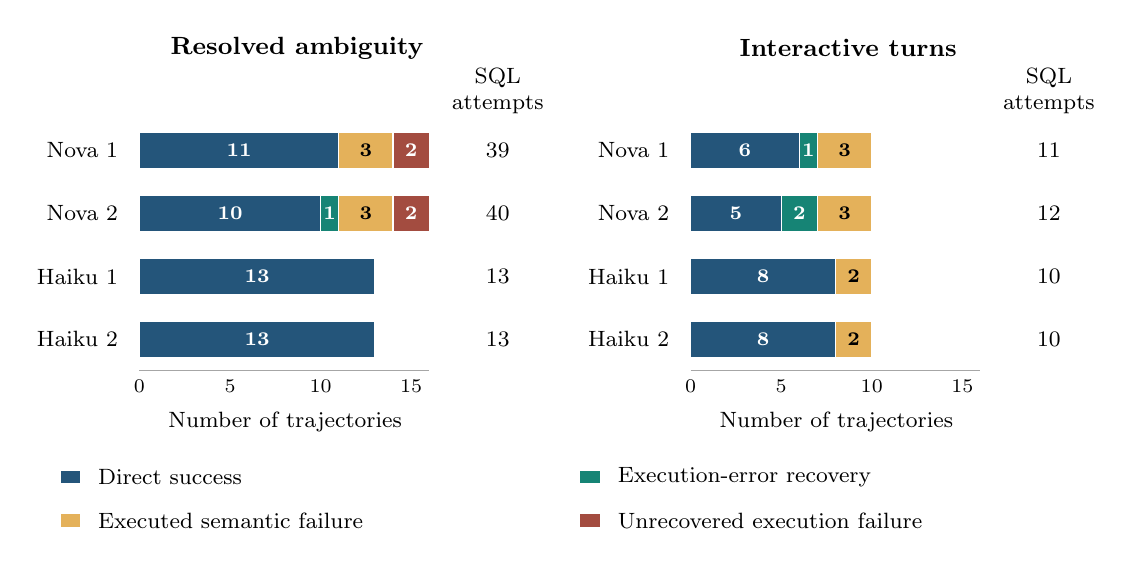
\begin{tikzpicture}[font=\footnotesize]
\node[font=\small\bfseries] at (3,1.3) {Resolved ambiguity};
\node[align=center] at (5.55,.75) {SQL\\attempts};
\node[anchor=east] at (0.85,0.0) {Nova 1};
\filldraw[fill=direct,draw=white,line width=.4pt] (1,-0.23) rectangle (3.5300000000000002,0.23);
\node[text=white,font=\scriptsize\bfseries,inner sep=0pt] at (2.265,0.0) {11};
\filldraw[fill=semantic,draw=white,line width=.4pt] (3.5300000000000002,-0.23) rectangle (4.220000000000001,0.23);
\node[text=black,font=\scriptsize\bfseries,inner sep=0pt] at (3.8750000000000004,0.0) {3};
\filldraw[fill=execution,draw=white,line width=.4pt] (4.220000000000001,-0.23) rectangle (4.680000000000001,0.23);
\node[text=white,font=\scriptsize\bfseries,inner sep=0pt] at (4.450000000000001,0.0) {2};
\node at (5.55,0.0) {39};
\node[anchor=east] at (0.85,-0.8) {Nova 2};
\filldraw[fill=direct,draw=white,line width=.4pt] (1,-1.03) rectangle (3.3000000000000003,-0.5700000000000001);
\node[text=white,font=\scriptsize\bfseries,inner sep=0pt] at (2.1500000000000004,-0.8) {10};
\filldraw[fill=recovery,draw=white,line width=.4pt] (3.3000000000000003,-1.03) rectangle (3.5300000000000002,-0.5700000000000001);
\node[text=white,font=\scriptsize\bfseries,inner sep=0pt] at (3.415,-0.8) {1};
\filldraw[fill=semantic,draw=white,line width=.4pt] (3.5300000000000002,-1.03) rectangle (4.220000000000001,-0.5700000000000001);
\node[text=black,font=\scriptsize\bfseries,inner sep=0pt] at (3.8750000000000004,-0.8) {3};
\filldraw[fill=execution,draw=white,line width=.4pt] (4.220000000000001,-1.03) rectangle (4.680000000000001,-0.5700000000000001);
\node[text=white,font=\scriptsize\bfseries,inner sep=0pt] at (4.450000000000001,-0.8) {2};
\node at (5.55,-0.8) {40};
\node[anchor=east] at (0.85,-1.6) {Haiku 1};
\filldraw[fill=direct,draw=white,line width=.4pt] (1,-1.83) rectangle (3.99,-1.37);
\node[text=white,font=\scriptsize\bfseries,inner sep=0pt] at (2.495,-1.6) {13};
\node at (5.55,-1.6) {13};
\node[anchor=east] at (0.85,-2.4000000000000004) {Haiku 2};
\filldraw[fill=direct,draw=white,line width=.4pt] (1,-2.6300000000000003) rectangle (3.99,-2.1700000000000004);
\node[text=white,font=\scriptsize\bfseries,inner sep=0pt] at (2.495,-2.4000000000000004) {13};
\node at (5.55,-2.4000000000000004) {13};
\node[font=\scriptsize] at (1.0,-3) {0};
\node[font=\scriptsize] at (2.1500000000000004,-3) {5};
\node[font=\scriptsize] at (3.3000000000000003,-3) {10};
\node[font=\scriptsize] at (4.45,-3) {15};
\draw[black!35] (1,-2.8) -- (4.68,-2.8);
\node at (2.85,-3.45) {Number of trajectories};
\node[font=\small\bfseries] at (10,1.3) {Interactive turns};
\node[align=center] at (12.55,.75) {SQL\\attempts};
\node[anchor=east] at (7.85,0.0) {Nova 1};
\filldraw[fill=direct,draw=white,line width=.4pt] (8,-0.23) rectangle (9.38,0.23);
\node[text=white,font=\scriptsize\bfseries,inner sep=0pt] at (8.690000000000001,0.0) {6};
\filldraw[fill=recovery,draw=white,line width=.4pt] (9.38,-0.23) rectangle (9.610000000000001,0.23);
\node[text=white,font=\scriptsize\bfseries,inner sep=0pt] at (9.495000000000001,0.0) {1};
\filldraw[fill=semantic,draw=white,line width=.4pt] (9.610000000000001,-0.23) rectangle (10.3,0.23);
\node[text=black,font=\scriptsize\bfseries,inner sep=0pt] at (9.955000000000002,0.0) {3};
\node at (12.55,0.0) {11};
\node[anchor=east] at (7.85,-0.8) {Nova 2};
\filldraw[fill=direct,draw=white,line width=.4pt] (8,-1.03) rectangle (9.15,-0.5700000000000001);
\node[text=white,font=\scriptsize\bfseries,inner sep=0pt] at (8.575,-0.8) {5};
\filldraw[fill=recovery,draw=white,line width=.4pt] (9.15,-1.03) rectangle (9.610000000000001,-0.5700000000000001);
\node[text=white,font=\scriptsize\bfseries,inner sep=0pt] at (9.38,-0.8) {2};
\filldraw[fill=semantic,draw=white,line width=.4pt] (9.610000000000001,-1.03) rectangle (10.3,-0.5700000000000001);
\node[text=black,font=\scriptsize\bfseries,inner sep=0pt] at (9.955000000000002,-0.8) {3};
\node at (12.55,-0.8) {12};
\node[anchor=east] at (7.85,-1.6) {Haiku 1};
\filldraw[fill=direct,draw=white,line width=.4pt] (8,-1.83) rectangle (9.84,-1.37);
\node[text=white,font=\scriptsize\bfseries,inner sep=0pt] at (8.92,-1.6) {8};
\filldraw[fill=semantic,draw=white,line width=.4pt] (9.84,-1.83) rectangle (10.3,-1.37);
\node[text=black,font=\scriptsize\bfseries,inner sep=0pt] at (10.07,-1.6) {2};
\node at (12.55,-1.6) {10};
\node[anchor=east] at (7.85,-2.4000000000000004) {Haiku 2};
\filldraw[fill=direct,draw=white,line width=.4pt] (8,-2.6300000000000003) rectangle (9.84,-2.1700000000000004);
\node[text=white,font=\scriptsize\bfseries,inner sep=0pt] at (8.92,-2.4000000000000004) {8};
\filldraw[fill=semantic,draw=white,line width=.4pt] (9.84,-2.6300000000000003) rectangle (10.3,-2.1700000000000004);
\node[text=black,font=\scriptsize\bfseries,inner sep=0pt] at (10.07,-2.4000000000000004) {2};
\node at (12.55,-2.4000000000000004) {10};
\node[font=\scriptsize] at (8.0,-3) {0};
\node[font=\scriptsize] at (9.15,-3) {5};
\node[font=\scriptsize] at (10.3,-3) {10};
\node[font=\scriptsize] at (11.45,-3) {15};
\draw[black!35] (8,-2.8) -- (11.68,-2.8);
\node at (9.85,-3.45) {Number of trajectories};
\fill[direct] (0,-4.23) rectangle (0.25,-4.07);
\node[anchor=west] at (0.35,-4.15) {Direct success};
\fill[recovery] (6.6,-4.23) rectangle (6.85,-4.07);
\node[anchor=west] at (6.949999999999999,-4.15) {Execution-error recovery};
\fill[semantic] (0,-4.78) rectangle (0.25,-4.62);
\node[anchor=west] at (0.35,-4.7) {Executed semantic failure};
\fill[execution] (6.6,-4.78) rectangle (6.85,-4.62);
\node[anchor=west] at (6.949999999999999,-4.7) {Unrecovered execution failure};
\end{tikzpicture}
\endgroup
